\documentclass[a4paper]{scrreprt}

\usepackage[T1]{fontenc}
\usepackage[utf8]{inputenc}
\usepackage[ngerman]{babel}
\usepackage{amsthm}
\usepackage{amsmath}
\usepackage{amssymb}
\usepackage{csquotes}
\usepackage{tikz}
\usepackage{graphicx}

% verlinktes Inhaltsverzeichnis
\usepackage[pdftex,
colorlinks=false]{hyperref}
\usepackage[all]{hypcap}

\newtheorem{definition}{Definition}

\DeclareMathOperator{\zeit}{zeit}
\DeclareMathOperator{\aktion}{aktion}

\setlength\parindent{0pt}

\newcommand\circlearound[1]{%
	\tikz[baseline]\node[draw,shape=circle,anchor=base] {#1} ;}

\title{Skript: Thread Programmierung, HTWK}
\subtitle{Gehalten von Prof. Geser im Sommersemester 2016}
\author{Lukas Werner \and Ann Kathrin Hartmann \and Toni Pohl \and Stephan Kemper}
\date{\today}

\begin{document}
	
\maketitle

\tableofcontents

\chapter{Grundbegriffe}

\section{Threads}

\begin{definition}[Prozess]
Sequentieller Rechenvorgang
\end{definition}

\begin{definition}[sequentiell]
Alle Rechenschritte laufen nacheinander in einer vorgegebenen Reihenfolge ab.
\end{definition}

\begin{definition}[Thread]
"`leichte"' Variante eines Prozesses
\end{definition}

Allgemeine Tendenz:
\begin{enumerate}
\item Systemkern möglichst "`schlank"' halten
\item Systemkern möglichst selten betreten
\end{enumerate}

Unterschied zu Prozess:
\begin{itemize}
\item Kein eigener Speicherbereich
\item Üblicherweise nicht vom Systemkern verwaltet ("`leight-weight process"'), vom Systemkern verwaltet
\end{itemize}

Vorteile:
\begin{itemize}
\item Wechsel zwischen Threads weniger aufwändig als Wechsel zwischen Prozessen
\item Threads benötigen weniger Speicher
\item Man kann viel mehr Threads ($\approx$ 10.000) als Prozesse ($\approx$ 100) laufen lassen.
\end{itemize}

Nachteil:\\
Anwendungsprogrammierer muss sich um Verwaltung der Threads kümmern.\\
\\
Viele Programmiersprachen bieten heutzutage Programmbibliotheken für Threads an (Beispiel: \emph{PThread} in C). Wir verwenden in dieser Veranstaltung \emph{Java} als Programmiersprache.

\begin{definition}[parallel]
Mehrere Threads laufen gleichzeitig auf verschiedenen Rechnerkernen.
\end{definition}

\begin{definition}[verschränkt (engl. interleaved)]
Threads laufen abwechselnd je ein Stück weit.
\end{definition}

\begin{definition}[nebeneinander laufend (auch: nebenläufig, engl. concurrent)]
Mehrere Threads laufen parallel oder miteinander verschränkt.
\end{definition}

Auch Mischformen sind möglich.\\
\\
Unterschied:\\
\begin{definition}[Rechenzeit (cpu time)]
Zeit, die der Prozessor mit Rechnen zubringt.
\end{definition}

\begin{definition}[Bearbeitungszeit (wall clock time)]
Umfasst auch Wartezeiten
\end{definition}

\subsubsection*{Amdahlsches Gesetz (Gene Amdahl, 1967):}
Wenn eine Aufgabe die Bearbeitungszeit $ a $ benötigt und der Anteil $ 0 \leq p \leq 1 $ davon parallelisierbar ist, dann benötigt sie auf $ n $ Prozessoren die Bearbeitungszeit

\begin{equation}
a \left( 1 - p + \frac{p}{n} \right).
\end{equation}

Beispiel:\\
$ p = \frac{9}{10} $, $ n = 100 $\\
\\
Beschleunigung (speed up): 
\begin{equation*}
 \frac{a}{a \left( 1 - p + \frac{p}{n} \right)} = \frac{1}{1 - \frac{9}{10} + \frac{9}{1000}} \approx 9,17
\end{equation*}

\begin{equation*}
\text{Sogar} \lim\limits_{n \to \infty} \frac{1}{1 - p + \frac{p}{n}} = \frac{1}{1 - p} = 10
\end{equation*}

Fazit: Der nicht-parallelisierbare Anteil dominiert die Bearbeitungszeit.

\section{Nicht-Determinismus}
\begin{definition}[Nicht-Determinismus]
Das Verhalten eines Systems hat Freiheitsgrade.
\end{definition}

Nicht-Determinismus hat zwei Anwendungen:
\begin{enumerate}
\item Möglichkeiten des Verhaltens der Systemumgebung zusammenfassen (engl. don't know nondeterminism)
\item Spielraum für Implementierungen vorsehen (engl. don't care nondeterminism)
\end{enumerate}

Hier: System von Threads\\
Man muss davon ausgehen, dass die Rechenschritte der Threads beliebig miteinander verschränkt sind. Die Reihenfolge der Schritte eines Threads ist durch sein Programm vorgegeben ("`Programm-Reihenfolge"').\\
Der Zeitplaner (engl. scheduler) legt zur Laufzeit fest, in welcher Reihenfolge die Schritte zweier Threads zueinander ablaufen. Man möchte den Zeitplaner in seiner Entscheidungsfreiheit nicht unnötig einschränken, sondern einen möglichst großen Spielraum lassen.\\
Man verlangt deshalb, dass das System von Threads korrekt zusammenarbeitet unabhängig davon, wie der Zeitplaner die Verschränkung bildet. Don't know nondeterminism aus der Sicht des Anwendungsprogrammierers, don't care nondeterminism aus der Sicht des Zeitplaners.\\
\\
Beispiel:\\
Thread 1 führt aus: \circlearound{1} \circlearound{2} \circlearound{3}\\
Thread 2 führt aus: \circlearound{a} \circlearound{b} \circlearound{c}\\
\\
Beispiele für mögliche Abläufe:
\begin{itemize}
\item \circlearound{1} \circlearound{a} \circlearound{2} \circlearound{b} \circlearound{3} \circlearound{c}
\item \circlearound{a} \circlearound{b} \circlearound{c} \circlearound{1} \circlearound{2} \circlearound{3}
\item \circlearound{a} \circlearound{1} \circlearound{2} \circlearound{3} \circlearound{b} \circlearound{c}
\item . . .
\end{itemize}

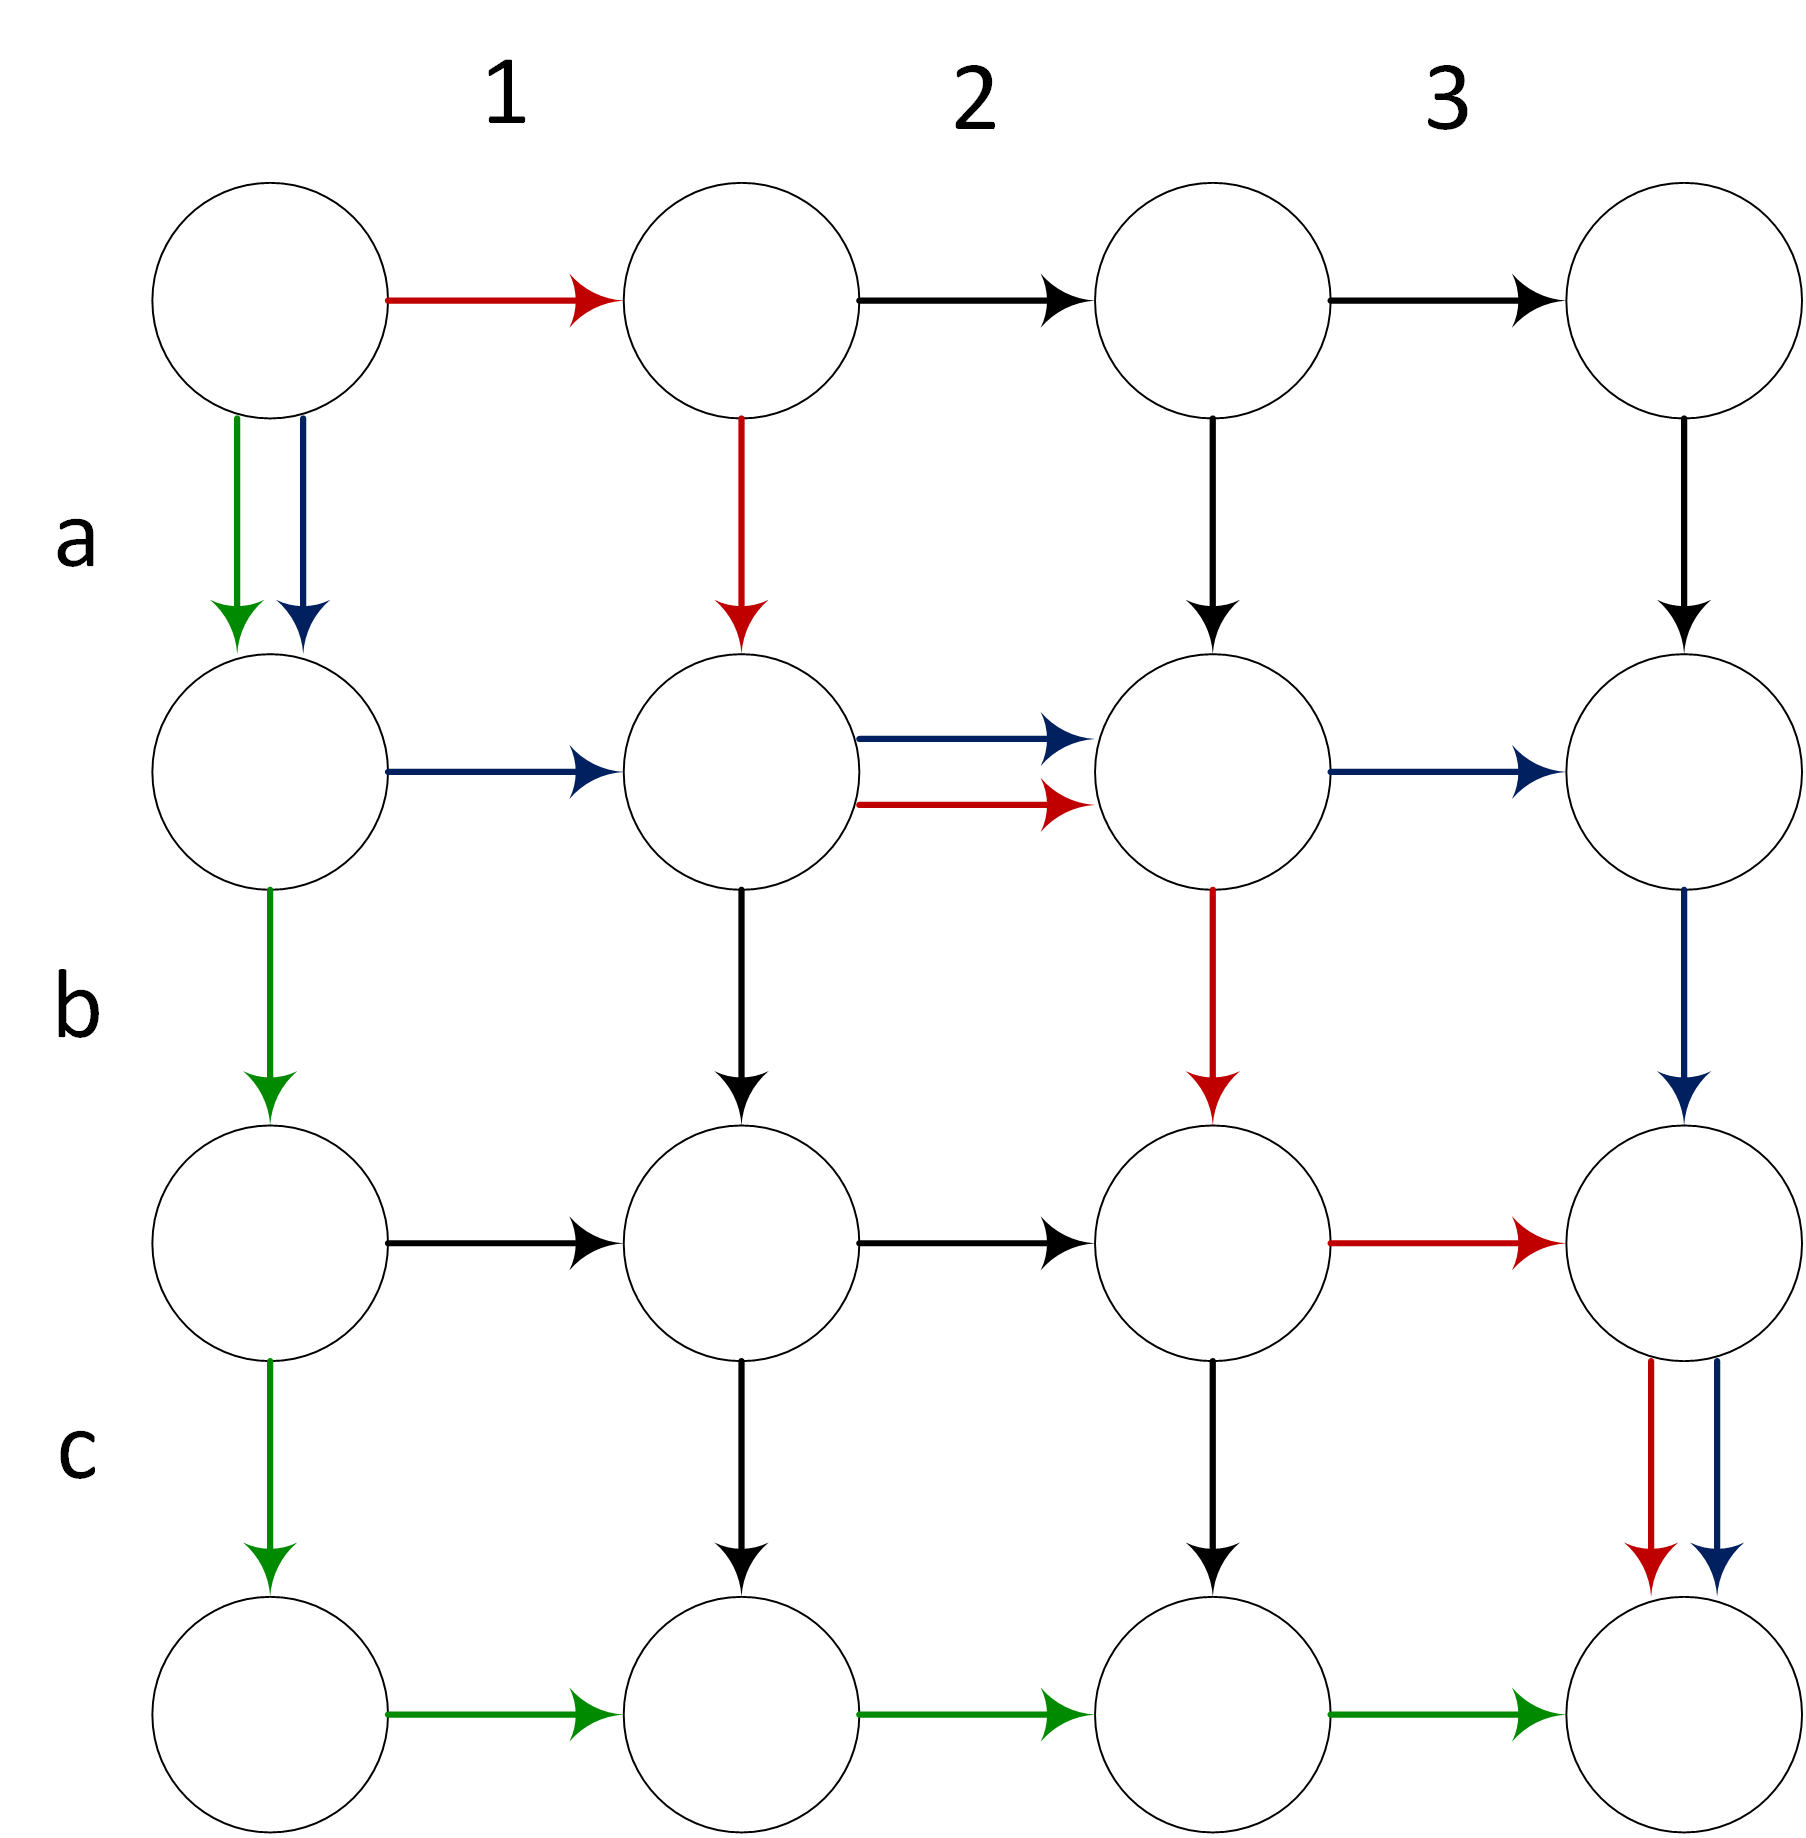
\includegraphics[width=.4\textwidth]{Nondeterminism}

Da bei jedem Test der Zeitplaner eine andere Ausführungsreihenfolge (Umstände des Wettrennens, engl. race conditions) wählen kann, ist der Test praktisch nicht reproduzierbar. Wegen der großen Anzahl möglicher Abläufe ist ein systematisches Testen aussichtslos ("`Zustandsexplosion"').
\chapter{Verifikation}

\section{Zeitliche Abläufe}
Vorgeben: Menge A von Aktionen
\begin{description}
\item {Ereignis (hier)} Paar bestehend aus Aktion und Zeitpunkt\\aktion(e), zeit(e) für Ereignis e.
\end{description}
Beispiel: Schlacht bei Isis 333 v. Chr. $\rightarrow$ Aktion, Zeitpunkt
\subsubsection*{Idealisierende Annahmen:}
\begin{enumerate}
\item Alles findet praktisch am selben Ort statt, keine Probleme mit der Lichtgeschwindigkeit (30cm in 1ns).
	\begin{description}
	\item[Zeit (hier)] Newtonsche Zeit, Sie verläuft
		\begin{itemize}
		\item absolut d.h. unabhängig von Beobachter (sonst: spezielle Relativitätstheorie)
		\item stetig, d.h. ohne Sprünge (sonst Quantenmechanik)
		\item unbeeinflusst von der Umgebung (sonst: allg. Relativitätstheorie)
		\item Zeitpunkt = reale Zahl
		\end{itemize}
	\end{description}
\item Ein Ereignis hat die Dauer Null. Einen Zeitraum kann man darstellen durch die Ereignisse “Ende des Zeitraums“.
\item Gleichzeitige Ereignisse sind ausgeschlossen, d.h. zwei Ereignisse, die die zur gleichen Zeit stattfinden, sind gleich\\
$zeit(e)1 = zeit(e2) \leftrightarrow e1 = e2 $
\end{enumerate}

\begin{description}
	\item[diskreter zeitlicher Ablauf (auch Geschichte)] Menge E von Ereignissen, so dass:
	\begin{enumerate}
		\item die Menge der Zeitpunkte E keinen Häufungspunkt hat
		\item die Menge der Zeitpunkte von E ein kleinstes Element hat
	\end{enumerate}
\end{description}

Sonst: kontinuierliche Vorgänge (reaktive Systeme).\\
Interessant sind hier nicht die Zeitpunkte selber, sondern nur deren Lage zueinander, d.h. die Reihenfolge der Aktionen. (Wenn dies nicht der Fall ist und Termine eingehalten werden müssen $ \rightarrow $ Echtzeitsystem)

\begin{description}
	\item[Def: (Leslie Lamport 1978)] Ereignis $ e_1 $ kommt vor Ereignis $ e_2 $ :\\
	$ e_1 \rightarrow e_2 \Leftrightarrow \zeit(e_1) < \zeit(e_2) $
\end{description}

Beispiel: Hochmut  $ \rightarrow $ Fall.\\
Es gilt: $ \rightarrow $ ist irreflexiv, transitiv, total, fundiert (d.h. eine Wohlordnung).

Eine Relation $ R \in E \times E $ auf der Menge $ E $ heißt
\begin{labeling}{xxxxxxxxxxxxx}
	\item[irreflexiv,] falls $ \forall e \in E $ gilt: $ (e, e) \notin  R $
	\item[transitiv,] falls $ \forall e_1, e_2, e_3 \in E $ gilt: Falls $ (e_1, e_2) \in R $ und $ (e_2, e_3) \in R $, dann $ (e_1, e_3) \in R $.
	\item[total,] falls $ \forall e_1, e_2 \in E $ gilt: Falls $ e_1 \neq e_2 $, dann $(e_1, e_2) \in R $ oder $ (e_2, e_1) \in R $
	\item[fundiert,] falls es keine unendliche Folge $ (e_i)_{i \in \mathbb{N}} $ gibt mit $ e_i \in E $ für alle $ i \in \mathbb{N} $ und $ (e_i, e_{i + 1}) \in R $ für alle $ i \in \mathbb{N} $
\end{labeling}

Einschub: R azyklisch, falls es keine endliche Folge $ (e_1, ..., e_n) $ gibt mit $ (e_1, e_2) \in R, (e_2, e_3) \in R, ..., (e_{n - 1}, e_n) \in R, (e_n, e_1) \in R $.
Falls $ R $ irreflexiv und transitiv ist, dann ist $ R $ auch azyklisch.

Für einen nicht-leere Geschichte $ E $ sei $ \min \ E $ definiert als das kleinste Element von $ E $ bezüglich $ \rightarrow $, d.h. dasjenige $ e \in E $ für das gilt:

\begin{equation*}
	\forall f \in E\setminus{e}: e \rightarrow f
\end{equation*}

Tipp: Relation als Graph vorstellen mit Wegen.
\begin{itemize}
	\item Es existiert kein Weg der Länge 1 zu sich selber.
	\item Wenn es einen Weg von 1 zu 2 und 2 zu 3 gibt, dann existiert eine Abkürzung von 1 zu 3.
	\item Es gibt immer Weg von jedem zu jedem Knoten.
	\item Es existiert kein unendlicher Weg.
\end{itemize}

\begin{description}
	\item[Implizite Definition] Definition durch eine charakterisierende Eigenschaft.
	\item[Wohldefiniertheit der implizierten Definition] Es gibt genau ein Objekt, dass die charakterisierende Eigenschaft erfüllt.
	(Beispiel: "`Wurzel von x ist das, was quadriert x ergibt"' ist nicht eindeutig (gar keine Lösung bzw. mehrere))
\end{description}

Wohldefiniertheit von min E gilt, weil $ R $ total und E (mindestens) ein kleinstes Element hat ($ \mathbb{Z} $ sind z.B. total auf $ < $, haben aber kein kleinstes Element).

Das i-te Element aus E ($ E^i $) ist dann für $ i \in \mathbb{N}, i \leq |E| $:
\begin{equation*}
	E^i := \begin{cases}
		\min \ E & \text{falls } i = 1\\
		(E \setminus{\min \ E})^{i - 1} & \text{sonst}
	\end{cases}
\end{equation*}

Auch hier ist Wohldefiniertheit zu zeigen.\\
Projektion auf eine Menge B von Aktionen ("`Sicht"'):
\begin{equation*}
	\pi_B(E) := e \in E | aktion(e) \in B
\end{equation*}
Zustand zum Zeitpunkt $ t \in R $:
\begin{equation*}
	z_t(E) := e \in E | zeit(e) \leq t % TODO: Kleiner oder kleiner gleich?!
\end{equation*}

$ \rightarrow $ für Zeiträume: Ende von Zeitraum A kommt vor Anfang von Zeitraum B: A $ \rightarrow $ B. Es gilt: Für Zeiträume ist $ \rightarrow $ \emph{nicht} total!
$ A \rightarrow B \vee B \rightarrow A \Leftrightarrow A $ und $ B $ überlappen nicht (Wenn sich $ A $ und $ B $ überlappen gilt weder $ A  \rightarrow B $ noch $ B \rightarrow A $).

\begin{description}
	\item[Prozessalphabet] Menge der Aktionen, die der Thread p "`sieht"'
	\item[Gemeinsame Aktionen von $ p_1 $ und $ p_2 $] $ \alpha(p_1) \cap \alpha(p_2) $
	\item[Einigkeit (engl. match)] Ereignisse mit gemeinsamen Aktionen finden gemeinsam statt:
	\begin{itemize} % TODO: Besser formatieren
		\item (1) $ \pi_{\alpha(p_1) \cap \alpha(p_2)}(E_1 \cup E_2 = E_1 \cap E_2 $ Gleichwertig zu (1) sind:\\
		\item (2) $ \pi_{\alpha(p_1) \cap \alpha(p_2)}(E_1 \oplus E_2 = \emptyset $ // symmetrische Differenz: Vereinigung ohne Schnitt
		\item (3) $ \pi_{\alpha(p_1)} = \pi_{\alpha(p_2)} $
	\end{itemize}
	\item[$ E_i $ Ereignis von Thread i] Es gilt: $ \forall e \in E_i: \aktion(e) \in \alpha(p_i) $
	\item[Faire Mischung] $ E_1 \cup E_2 $
	\item[Gemeinsame Ereignisse] $ \pi_{\alpha(p_i)}(E_1 \cap E_2) = E_i, für i \in {1, 2} $, falls sich $ p_1 $ und $ p_2 $ einig sind. Es gilt: $ E_1 \cup E_2 $.
\end{description}


\section{Serielle Abläufe}
Wenn man nicht an den Zeitpunkten der Ereignisse interessiert ist, sondern nur an ihrer Lage zueinander, kann man statt einer Ereignismenge auch eine Aktionenfolge als Beschreibungsmittel für einen Ablauf nehmen.

Beispiele: Sei $ A = \{a, b\} $. Endliche Folge $ (a, b, a) $ kann auch dargestellt werden als Funktion $ f: {1, 2, 3} \rightarrow A $ mit $ f(x) = \begin{cases} a & \text{falls } x = 1 \vee x = 3\\ b & \text{sonst}\end{cases} $\\
Wertetabelle von f:
\begin{center}
	\begin{tabular}{l|c c c}
		$ x $ & 1 & 2 & 3\\ \hline
		$ f(x) $ & a & b & c
	\end{tabular}
\end{center}

Unendliche Folge $ (a, b, b, a, b, b, ...) $ als Funktion $ f: \mathbb{N} \rightarrow A $ mit $ f(x) = \begin{cases} a & \text{falls } x \mod 3 = 1\\ b & \text{sonst}\end{cases} $\\
\\
$ A^k $ k-Tupel von Elementen aus A und \\
$ {i \in \mathbb{N} | i \leq k} \rightarrow A $ Folgen der Länge k werden miteinander identifiziert.

\section{Faire Mischung}

\section{Sicherheits- und Liveness-Eigenschaften}

\section{Modellierung}
\chapter{Synchronisation}

\section{Signale}
\begin{description}
\item[Synchronisation (hier)] Dafür sorgen, dass gewisse Abläufe ausgeschlossen sind.\\
Auch: Koordination.
\item[Signal (auch: Handshake, Meldung, engl. notification)] Hinweis an einen anderen Thread, dass er weitermachen kann.
\end{description}

Analogie:
\begin{itemize}
	\item Startschuss beim Wettlauf
	\item Staffel beim Staffellauf
	\item Anschlusszug muss warten
	\item Becher vor Kaffeezulauf
\end{itemize}

Ein Signal kann durch eine Sperre implementiert werden: 
\begin{itemize}
	\item signalisieren (auch: melden) = freigeben
	\item warten = belegen
\end{itemize}
Das Signal soll garantieren, dass eine gewisse Reihenfolge eingehalten wird.\\
\\ % TODO: Einrücken
P1: S1;
	freigeben(l);
P2:	belegen(l);
	S2;\\
% TODO: Grafik 20160519_SynchronisationZeitstrahl einfügen
\\
l muss freigegeben worden sein, bevor es wieder belegt werden kann, also findet S1 vor S2 statt.\\
\\
Durch die Verwendung von Signalen schränkt man die Menge der Abläufe ein.\\
Nachteil: weniger Parallelität\\
Extremfall: Nur noch eine Reihenfolge möglich; der Ablauf wird seriell. Abgesehen vom Koordinationsaufwand zu einem seriellen Programm gleichwertig.

\section[Beispiel: Erzeuger/Verbraucher (1)]{Beispiel: Erzeuger/Verbraucher-Problem, 1. Version}
Erzeuger und Verbraucher sind Threads. Der Erzeuger erzeugt Datenblöcke. Der Verbraucher holt die Datenblöcke ab und verarbeitet sie.\\
Die erzeugten aber noch nicht verbrauchten Datenblöcke werden in einem Puffer (:= Warteschlange) zwischengespeichert.\\
\\
\textbf{1. Version}: 1 Erzeuger, 1 Verbraucher, Puffer für 1 Datenblock.\\
\\ % TODO: Pseudocode
Thread erz:
	Wiederhole
		herstellen(datenblock);
		einreihen(puffer, datenblock);
Thread verbr:
	Wiederhole
		abholen(puffer, datenblock);
		verarbeiten(datenblock);\\
\\
Prozedur einreihen(puffer, datenblock):
\begin{enumerate}
	\item belegen(leer);
	\item kopieren(datenblock, puffer); $\rightarrow$ kopiert Datenblock in Puffer
	\item freigeben(voll);
\end{enumerate}
Prozedur abholen(puffer, datenblock):
\begin{enumerate}
	\setcounter{enumi}{3}
	\item belegen(voll);
	\item kopieren(puffer, datenblock); $\rightarrow$ kopiert Puffer in Datenblock
\end{enumerate}
Hauptprogramm (HP):
\begin{enumerate}
	\item[] Sperre voll anlegen; $\rightarrow$ als belegt
	\item[] Sperre leer anlegen; $\rightarrow$ als belegt
	\item[] Threads erz und verbr anlegen und laufen lassen;
	\item[0.] freigeben(leer);
\end{enumerate}

\subsubsection*{Kausalitätsgraph:} % TODO: Grafik Kausalitätsgraph

Ereignis $ e_1 $ \emph{ist kausal für} Ereignis $ e_2 $ $ :\Leftrightarrow $ In jedem Ablauf gilt: Wenn $ e_2 $ stattfindet, dann hat $ e_1 $ vorher stattgefunden. Mit anderen Worten: $ e_2 $ kann erst stattfinden, wenn $ e_1 $ vorher stattgefunden hat.

% Pfeil
Programmreihenfolge
% Gestrichelter Pfeil
Reihenfolge erzwungen durch Signal

\subsubsection*{Petri-Netz:} % TODO: Grafik Petrinetz
Legende für Petri-Netz: Kreis Platz, Strich Transition, Punkt Token.\\
\\
Bipartiter Graph: Zwei Sorten von Knoten; Pfeile nur zwischen verschiedenen Knoten-Sorten.
% TODO: Wenn möglich, Petrinetz laufen lassen

\subsubsection*{Signaldiagramm}

% TODO Grafik Signaldiagramm

Verwendung der Sperren voll und leer bewirkt hier:
\begin{enumerate}
\item (2) und (5) werden als kritische Bereiche behandelt. 
\item (2) und (5) werden nur abwechselnd ausgeführt.
\end{enumerate}
zu 1: Gegenseitiger Ausschluss gilt. $ \neg $leer.frei $\lor$ $\neg$voll.frei ist Invariante.\\
zu 2: Folgt aus Programmreihenfolge und 1.

\section{Semaphore}

\begin{description}
\item[Semaphor] Datenstruktur l mit Zustand l.frei $ \in \mathbb{N_0} $ und Operationen "`belegen"' und "`freigeben"'.
\end{description}
Sperre ist Spezialfall mit l.frei $ \in \{0, 1\} $.\\
\\
belegen(l): Wartet bis l.frei > 0 und setzt dann l.frei auf l.frei - 1.\\
freigeben(l): setzt l.frei auf l.frei + 1.\\
\\
Zweck: l.frei verschiedene Kopien eines Betriebsmittels werden verwaltet.\\
\\
Zusammenhang zu Klammerausdrücken:\\
"`("' bedeutet "`freigeben(l)"'\\
"`)"' bedeutet "`belegen(l)"'\\
l.frei = Anzahl der noch offenen Klammern.\\
\\
Beispiel:          ( ( ) ( ) ) % TODO Zeitstrahl
%l.frei 2_|           _   _
%       1_|         _| |_| |_
%         |________|         |_______
%

\section[Beispiel: Erzeuger/Verbraucher (2)]{Beispiel: Erzeuger/Verbraucher-Problem, 2. Version}
2. Version: 1 Erzeuger, 1 Verbraucher, N Datenblöcke mit $ N > 0 $ beliebig.\\
\\
Threads erz und verbr wie in Version 1.\\
\\
Prozedur einreihen(puffer, datenblock):
\begin{enumerate}
\item belegen(nichtvoll);$ \rightarrow $ \textbf{I' gilt nun wieder}
\item stock(puffer, datenblock); $ \rightarrow $ Anfügen des Datenblocks an Puffer hinten
\item freigeben(nichtleer);$ \rightarrow $ \textbf{I gilt}
\end{enumerate}
Prozedur abholen(puffer, datenblock):
\begin{enumerate}
\setcounter{enumi}{3}
\item belegen(nichtleer); $\rightarrow$ \textbf{I' gilt}
\item datenblock := top(puffer); $ \rightarrow $ liefert vordersten Datenblock des Puffer
\item pop(puffer);
\item freigeben(nichtvoll); $\rightarrow$ \textbf{I gilt}
\end{enumerate}
Hauptprogramm:
\begin{itemize}
\item Leeren puffer anlegen
\item Semaphore nichtvoll und nichtleer erzeugen mit nichtvoll.frei = 0 und nichtleer.frei = 0.
\item Threads erz und verbr anlegen und laufen lassen.
\item freigeben$^N$(nichtvoll); $\rightarrow$ nichtvoll wird N-mal freigegeben. 
\item \textbf{I gilt}
\end{itemize}

Invariante I: $ 0 \leq \text{ nichtvoll.frei } \leq N \land \text{ nichtleer.frei } + \text{ nichtvoll.frei } \leq N $\\
Invariante I': $ 0 \leq \text{ nichtvoll.frei } \leq N \land \text{ nichtleer.frei } + \text{ nichtvoll.frei } \leq N - 1 $\\
Invariante I'': $ 0 \leq \text{ nichtvoll.frei } \leq N \land \text{ nichtleer.frei } + \text{ nichtvoll.frei } \leq N - 2 $\\
I'' gilt, wenn beide Threads belegen, aber noch nicht freigeben aufgerufen haben.

\section{Bedingte kritische Bereiche}
Ein kritischer Bereich soll nur betreten werden, wenn eine gewisse Bedingung B an die gemeinsame Variable gilt. Wie implementiert man das?
\begin{enumerate}
\item B vor dem Betreten des kritischen Bereichs überprüfen.\\Problem: B kann beim Betreten des kritischen Bereiches bereits wieder verletzt sein.
\item B im kritischen Bereich überprüfen.\\Problem: Solange B nicht gilt, soll der Thread warten. Weil er sich im kritischen Bereich befindet, können andere Threads die gemeinsame Variable nicht ändern und damit den Wert von B.
\end{enumerate}
Mit kritischen Bereichen kann man das Problem nicht lösen. Abhilfe: neues Konstrukt.

\section[Beispiel: Erzeuger/Verbraucher (3)]{Beispiel: Erzeuger/Verbraucher-Problem, 3. Version}

\section{Wiederbetretbare Sperren}

\section{Leser/Schreiber-Problem}
\chapter{Feinkörnige Nebenläufigkeit}
Problem: Bei einem hohen Grad an Nebenläufigkeit wird der Zugriff auf das gemeinsame Objekt zum Flaschenhals. Die Threads können nur nacheinander zugreifen.\\
Abhilfe: 4 Techniken.
\begin{enumerate}
	\item \textbf{Feinkörnige Synchronisation:} Statt das Objekt zu sperren, werden nur die betroffenen Komponenten gesperrt. Nur wenn zwei Threads auf dieselbe Komponente zugreifen wollen, muss einer warten.
	\item \textbf{Optimistische Synchronisation:} Während der Suche nach einer bestimmten Komponente des Objekts werden keine Sperren erworben. Sobald die Komponente gefunden wurde, diese Komponente sperren und überprüfen, ob sich der Kontext inzwischen verändert hat.
	\item \textbf{Faule Synchronisation:} Löschen einer Komponente wird in zwei Phasen durchgeführt:
	\begin{enumerate}
		\item Als gelöscht markieren, z.B. durch Setzen eines gewissen Bits ("`logisches Löschen"').
		\item Aus der Datenstruktur aushängen ("`physikalisches Löschen"').
	\end{enumerate}
	\item \textbf{Nicht-blockierende Synchronisation:} Statt Sperren werden atomare Operationen verwendet.
\end{enumerate}

\section[Mengen mit verketteten Listen]{Beispiel: Mengen implementiert durch verkettete Listen}
Mengen-Schnittstelle:
\begin{lstlisting}
Typ Set<T>
Methoden
    add(T x) // x zu Menge this hinzufuegen
    remove(T x) // x aus Menge this entfernen
    containes(T x) // Wahrheitswert von "this enthaelt x"
\end{lstlisting}
Implementierung von Mengen durch verkettete Listen mit Wächtern, sortiert nach Streuwert.\\
\\
Listenelement (Typ Node<T>) habe folgende Attribute:\\
\begin{description}
	\item[T item] das Element der Menge
	\item[int key] der Streuwert des Elements
	\item[Node<T> next] Zeiger auf das nächste Element
\end{description}

\begin{description}
	\item[Wächter (engl. Sentinel)] "`künstliches"' Listenelement, das Anfang oder Ende der Liste markiert.
\end{description}

Beispiel:
\begin{figure}[H]
	\begin{center}
		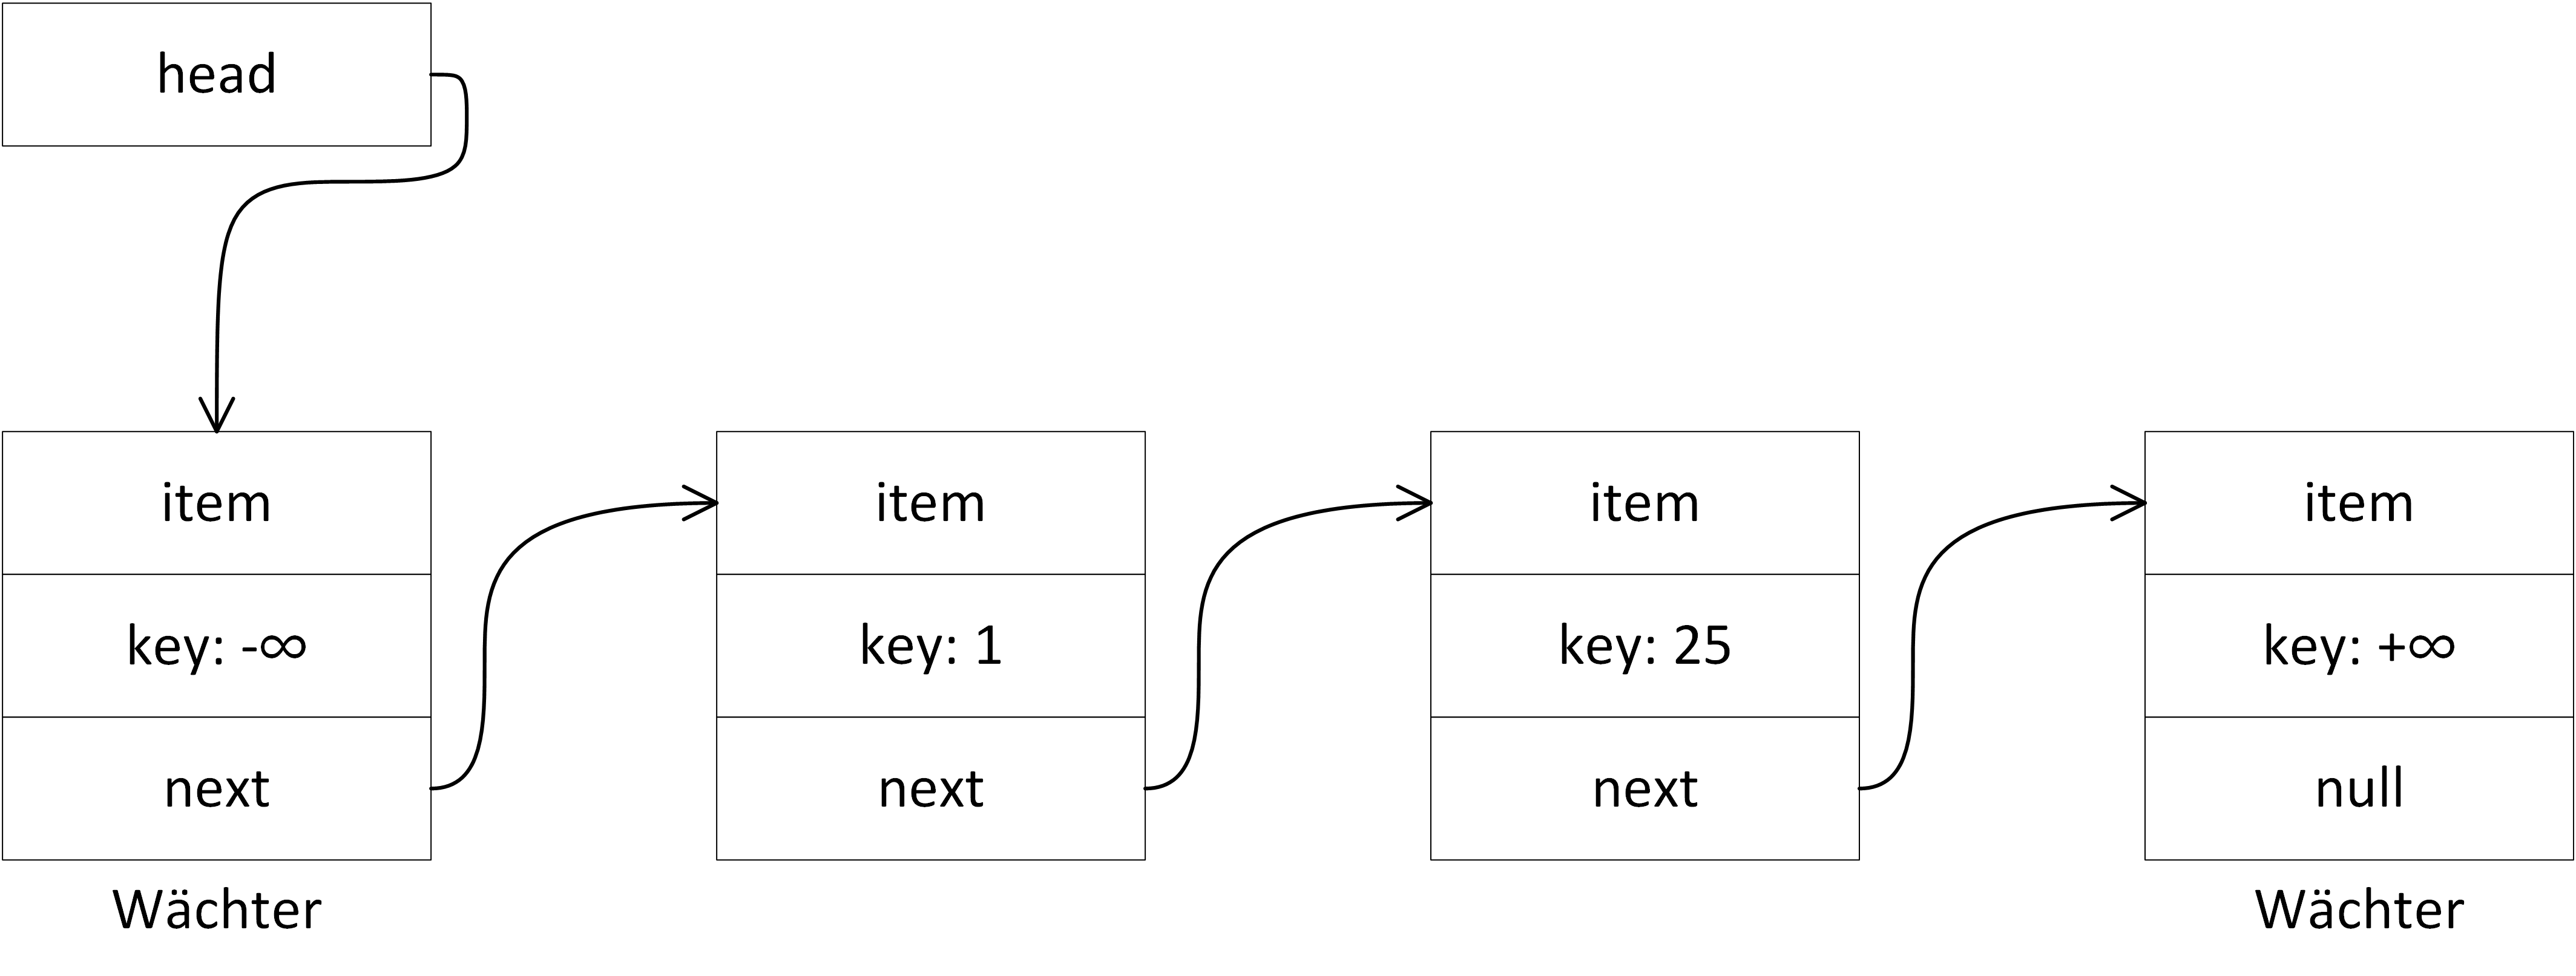
\includegraphics[width=\textwidth]{res/linkedlist}
		\caption{Visualisierung einer LinkedList.}
		\label{pic:linkedlist}
	\end{center}
\end{figure} 
Die Streuwerte sind sortiert: $ -\infty \leq 1 \leq 25 \leq +\infty $.\\
\\
Klasse List<T> mit Attribut head vom Typ Node<T>.\\
Invariante: Wächter werden weder hinzugefügt noch gelöscht. Die Listenelemente sind nach Streuwert sortiert.

\section{Implementierung mit Feinkörniger Synchronisation}
In Java:
\begin{lstlisting}
class List<T> {
	...
	public boolean add(T x) {
		int k = x.hashCode(); // Streuwert
		Node<T> pred, curr;
		try {
			pred = this.head;
			curr = pred.next;
			pred.lock(); // Assume implementation
			curr.lock();
			while (curr.key < k) {
				pred.unlock();
				pred = curr;
				curr = pred.next;
				curr.lock();
			}
			if (curr.key != k) {
				Node<T> node = new Node<>(x);
				node.next = curr;
				pred.next = node;
			}
		} finally {
			curr.unlock();
			pred.unlock();
		}
	}
}
\end{lstlisting}

Methoden remove und contains ähnlich.\\
\\
Eine Sperre genügt nicht. Beispiel dazu:
\begin{figure}[H]
	\begin{center}
		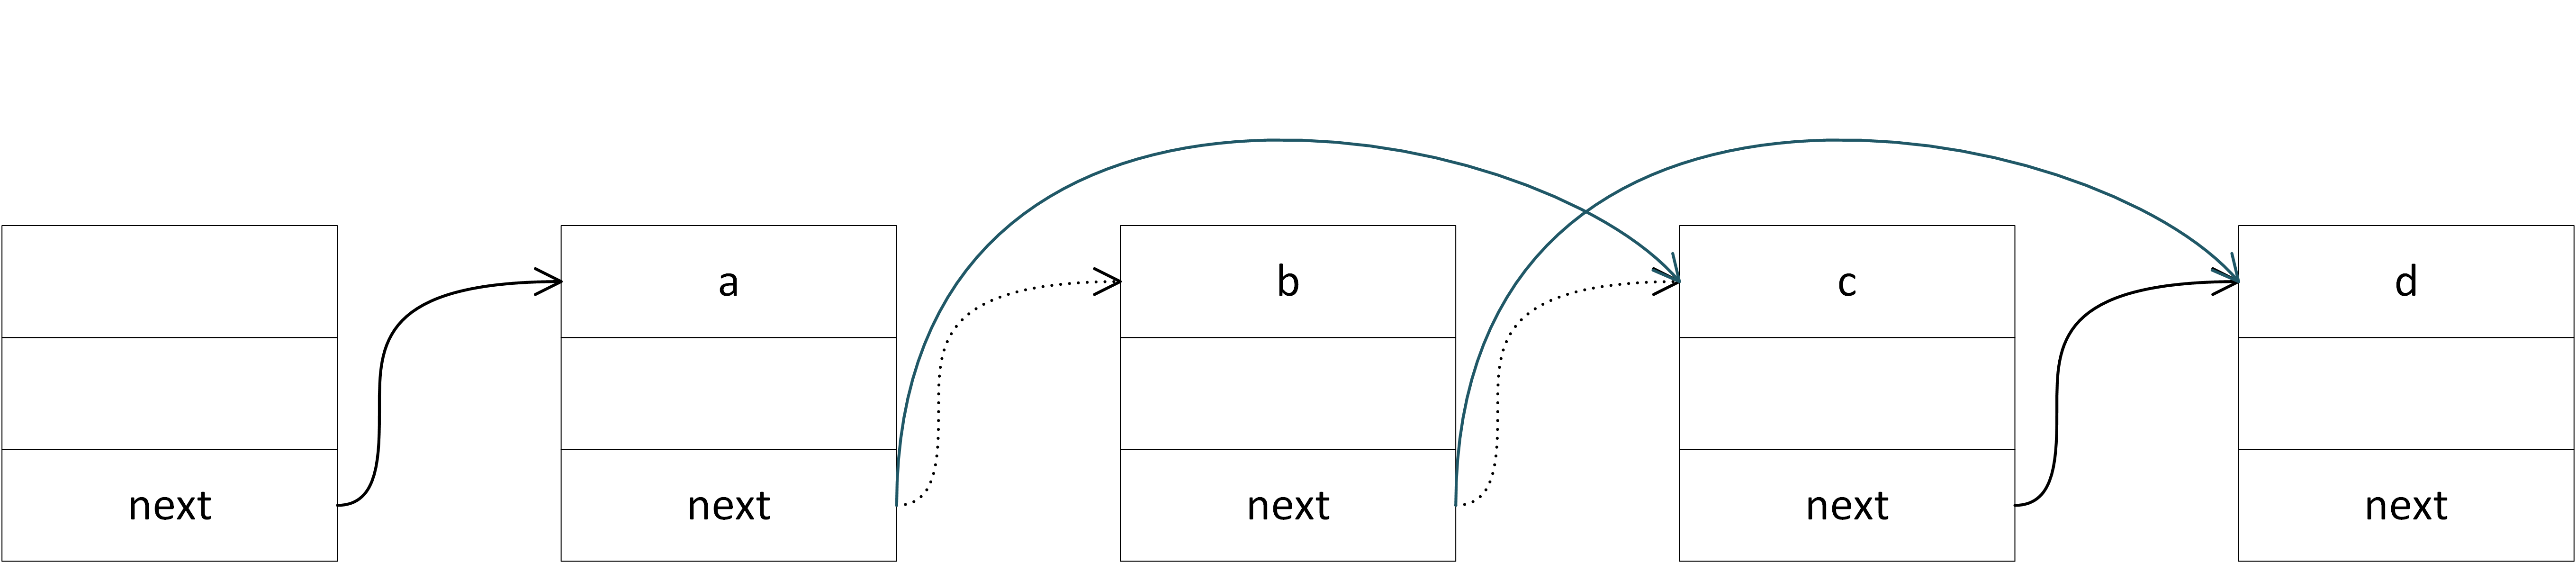
\includegraphics[width=\textwidth]{res/linkedlist_onelock}
		\caption{Visualisierung einer LinkedList.}
		\label{pic:linkedlistonelock}
	\end{center}
\end{figure} 
Thread 1 will b löschen:
\begin{itemize}
	\item Sperre in a erwerben
	\item a.next auf c setzen
\end{itemize}
Thread 2 will c löschen:
\begin{itemize}
	\item Sperre in b erwerben
	\item b.next auf d setzen
\end{itemize}
Wirkung: Nur b wird gelöscht!\\
\\
Um b zu löschen, muss die Sperre in a und in b erworben werden, und entsprechend um c zu löschen, muss die Sperre in b und in c erworben werden. $\Rightarrow$ Konflikt!

\pagebreak

\section{Implementierung mit optimistischer Synchronisation}

In Java:
\begin{lstlisting}
class OptList<T> {
	...
	public boolean add(T x) {
		int k = x.hashCode();
		Node<T> pred, curr;
		boolean done = false;
		while (!done) {
			pred = this.head;
			curr = pred.next;
			while (curr.key < k) {
				pred = curr;
				curr = pred.next;
			}
			try {
				pred.lock();
				curr.lock();
				if (this.validate(pred, curr)) {
					if (curr.key != k) {
						Node<T> node = new Node<>(x);
						node.next = curr;
						pred.next = node;
					}
					done = true;
				}
			} finally {
				curr.unlock();
				pred.unlock();
			}
		}
	}
	
	private boolean validate(Node<T> pred, Node<T> curr) {
		Node<T> node = this.head;
		while (node.key < pred.key) {
			node = node.next;
		}
		return node == pred && curr = node.next;
	}
}
\end{lstlisting}
Diskussion: Optimistisches Synchronisation lohnt sich, wenn zweimaliges Durchlaufen der Liste billiger ist als einmaliges Durchlaufen mit Setzen von Sperren. Belegen und Freigeben sind aufwendig.

\section{Implementierung mit fauler Synchronisation}
Listenelemente bekommen ein neues Attribut: \emph{marked} drückt aus, dass es zum Löschen markiert wurde.\\
\\
Neue Version von validate:
\begin{lstlisting}
private boolean validate(Node<T> pred, Node<T> curr) {
	return !pred.marked && !curr.marked && pred.next == curr;
}
\end{lstlisting}
Löschen:
\begin{lstlisting}
public boolean remove(T item) {
	int k = item.hashCode();
	boolean done = false;
	boolean erg = false;
	while (!done) {
		Node<T> pred = this.head;
		Node<T> curr = pred.next;
		while (curr.key < k) {
			pred = curr;
			curr = pred.next;
		}
		pred.lock();
		try {
			curr.lock();
			try { // falls erste Sperre geht, aber zweite nicht
				if (validate(pred, curr)) {
					if (curr.key == j) {
						curr.marked = true;
						pred.next = curr.next;
						erg = true;
					}
					done = true;
				}
			} finally {
				curr.unlock();
			}
		} finally {
			pred.unlock();
		}
	}
	return erg;
}
\end{lstlisting}
Contains:
\begin{lstlisting}
public boolean contains(T item) {
	int k = item.hashCode();
	Node<T> curr = this.head;
	while (curr.key < k) {
		curr = curr.next;
	}
	return curr.key == key && !curr.marked;
}
\end{lstlisting}
\chapter{Implementierung}

\section{Atomare Maschinenbefehle}
Wie werden Sperren implementiert?

\subsubsection*{Naiver Versuch}
\begin{lstlisting}
belegen(l):
	Solange !l.frei gilt, wiederhole:    (1)
		warte einen Augenblick;          (2)
	setze l.frei = false;                (3)
\end{lstlisting}
Beispielablauf für 2 Threads, die versuchen, belegen(l) aufzurufen. Sei zu Beginn l.frei = true.
\begin{center}
\begin{tabular}{c c|c}
$P_1$ & $P_2$ & l.frei \\ \hline
(1) & \ & \ \\ 
\ & (1) & \ \\ 
(3) & \ & \ \\
\ & (3) & \ 
\end{tabular}
\end{center}
$\rightarrow$ Beide Threads sind im kritischen Bereich!\\
$\Rightarrow$ (1)(2)(3) muss selber wieder ein kritischer Bereich sein.\\
\\
Man benötigt einen speziellen Maschinenbefehl, z.B.:
\begin{lstlisting}
getAndSet(c, b, v):
	b := c;
	c := v;
\end{lstlisting}
Zwei Ausführungen dieses Maschinenbefehls müssen immer unter gegenseitigem Ausschlusds stattfinden, d.h. der Maschinenbefehl muss atomar (komplett und unteilbar) sein. Die Hardware muss dafür sorgen ("`Arbitrierung"').

\subsubsection*{Implementierung mit getAndSet}
\begin{lstlisting}
belegen(l):
	boolean b;
	getAndSet(l.frei, b, false);
	solange !b wiederhole:
		warte einen Augenblick;
		getAndSet(l.frei, b, false);

freigeben(l):
	boolean b;
	getAndSet(l.frei, b, true);
\end{lstlisting}

\subsubsection*{Alternativen}

\begin{lstlisting}
getAndInc(c, b):
	b := c;
	c := c + 1;
	
getAndDec(c, b):
	b := c;
	c := c - 1;

compareAndSet(c, e, v, b): // b := Wahrheitswert
	Falls c = e, dann:
		c := v;
		b := true;
	Sonst:
		b := false;
\end{lstlisting}
(Befehl CMPXCHG (compare exchange) auf Intel Pentium)

\subsubsection*{Implementierung mit compareAndSet}

\begin{lstlisting}
belegen(l):
	boolean b;
	compareAndSet(l.frei, true, false, b);
	Solange !b wiederhole:
		warte einen Augenblick;
		compareAndSet(l.frei, true, false, b);

freigeben(l):
	boolean b;
	compareAndSet(l.frei, false, true, b);
\end{lstlisting}

\textbf{Volatile} (engl. für flüchtig), Schlüsselwort in Java.\\
Beispiel:
\begin{lstlisting}
volatile int x;
\end{lstlisting}
x ist damit als gemeinsame Variable gekennzeichnet. Übliche Optimierungen des Compilers für lokale Variablen sind ausgeschlossen. Lese- und Schreibzugriffe auf x sind zueinander atomar ("`atomares Register"'). Die Hardware sorgt für Atomarität.

\section{Konsenszahlen}

n-Konsens mit \emph{compareAndSet} und \emph{get}:\\
(Einfaches Konsensproblem: Jeder schlägt sich selber vor)\\
\begin{lstlisting}
init(c):
    Setze c = -1.

entscheide(c, i, a): // mit i: Thread-ID des Aufrufers
    boolean b;
    compareAndSet(c, -1, i, b);
    Falls b gilt, dann:
        a := i;
    Sonst:
        a := get(c); // Kann auch ohne Fallunterscheidung
                     // angewandt werden, da fuer b true gilt:
                     // i == get(c)
\end{lstlisting}

\subsubsection*{Read/Modify/Write-Operation:}
rmw(c, b, f): (mit c ist gemeinsame Variable mit Wert vom Typ T, b ist Ergebnisvariable mit Wert von Typ T und f ist Modifikationsfunktion f: T $\rightarrow$ T).\\
b := c;\\
c := f(c);\\

Es gilt: \\
getAndSet(c, b, v) = rmw(c, b, $\lambda$x . v)\\
getAndInc(c, b) = rmw(c, b, $\lambda$x . x + 1)\\

Schar F von Funktionen von T nach T heißt \emph{Common2}, falls:

\begin{align}
	f(g(x)) & = f(x) \text{ (f absorbiert g) oder}\\
	g(f(x)) & = g(x) \text{ oder}\\
	f(g(x) & = g(f(x))	
\end{align}
für alle $f, g \in F, x \in T$ (trivial für f = g).\\
\\
F heißt \emph{nicht-trivial}, falls $ F \neq \{id\} $ mit $ F $ ist nichtleer, d.h. $ F \backslash \{id\} \neq \emptyset $.\\
\\
Beispiel: $ F = \{\lambda x\ .\ x + 1, \lambda x\ .\ x - 1\} = \{s, p\} $.\\
Es gilt: $ s(p(x) = x = p(s(x)) $ für alle $ x \in \mathbb{Z} $. Also ist $ F $ Common2. Damit Konsenszahl $\leq$ 2. Da $ F $ nicht-trivial, ist Konsenszahl = 2. 

\section{Zwischenspeicher}

\begin{description}
	\item[Zwischenspeicher (ZSP, engl. cache)] schneller, kleiner Speicher auf dem Prozessorchip.
\end{description}
Bemerkung: Herkunft des Begriffs "`cache"': Versteck der Beute eines Einbrechers.\\
\\
Verwendung:\\
Nachdem der Prozessor das erste Mal auf eine gewisse Arbeitsspeicherzelle lesend zugegriffen hat, speichert er den Wert in seinem ZSP. Wenn er das nächste Mal lesend auf dieselbe Adresse zugreifen will, findet er das Ergebnis in seinem ZSP ("`Treffer"', engl. match). Er braucht dazu nicht auf den BUS zuzugreifen.

Um schreibend auf eine Arbeitsspeicherzelle zuzugreifen, speichert der Prozessor das Wort zunächst in seinen ZSP. Nur wenn ein anderer Prozessor auf dieselbe Speicherzelle lesend zugreifen will, muss das Wort in den Arbeitsspeicher geschrieben werden.

\subsubsection*{Vorteil des ZSP:}
Weniger Zugriffe auf den Arbeitsspeicher nötig, damit schneller und der BUS ist weniger belastet.

Der ZSP lohnt sich, wenn im Programm häufig dicht hintereinander Zugriffe auf dieselbe Adresse vorkommen ("`Lokalität"').

Um den Verwaltungsaufwand gering zu halten, ist der ZSP in sogenannte \emph{Speicherzeilen} (engl. cache lines) organisiert. Sobald der ZSP voll ist, wird es nötig, manche Zeilen auszuwerfen (engl. to evict) um Platz zu schaffen.

\begin{description}
	\item[Kohärenz] Jeder Lesezugriff auf den ZSP liefert den zuletzt geschriebenen Wert.
\end{description}

Kohärenz bedeutet praktisch, dass sich durch die Einführung des ZSP nichts am Verhalten des Systems ändert.

Um Kohärenz zu erreichen, verwendet man ein Kohärenz-Protokoll, z.B. das MESI-Protokoll.

\subsubsection*{MESI-Protkoll:}

Jede Speicherzeile hat einen Modus:
\begin{description}
	\item[Modified] Zeile wurde verändert. Kein anderer Prozessor hat diese Zeile in seinem ZSP.
	\item[Exclusive] Zeile ist unverändert. Kein anderer Prozessor hat diese Zeile in seinem ZSP.
	\item[Shared] Zeile ist unverändert. Andere Prozessoren können diese Zeile in ihrem ZSP haben.
	\item[Invalid] Zeile enthält eine verwertbaren Daten.
\end{description}
Beispiel-Ablauf:\\
A, B, C seien Prozessoren, M sei ein Arbeitsspeicherblock.
\begin{figure}[H]
	\begin{center}
		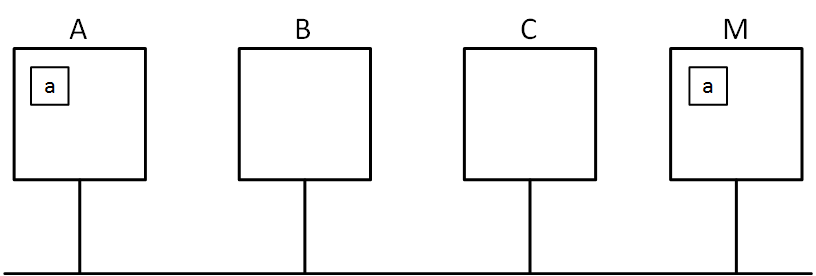
\includegraphics[width=.5\textwidth]{res/mesi_01}
		\caption{A liest Adresse von a.}
		\label{pic:mesi01}
	\end{center}
\end{figure} 
\begin{figure}[H]
	\begin{center}
		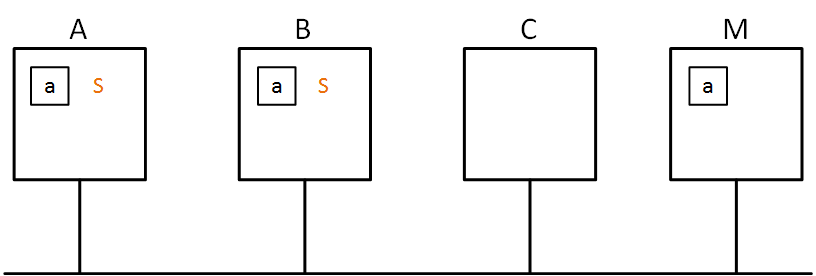
\includegraphics[width=.5\textwidth]{res/mesi_02}
		\caption{B liest Adresse von a; A antwortet.}
		\label{pic:mesi02}
	\end{center}
\end{figure} 
\begin{figure}[H]
	\begin{center}
		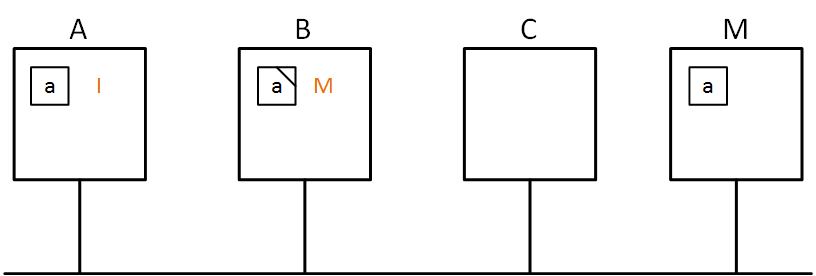
\includegraphics[width=.5\textwidth]{res/mesi_03}
		\caption{B schreibt auf Adresse a und informiert alle darüber.}
		\label{pic:mesi03}
	\end{center}
\end{figure} 
\begin{figure}[H]
	\begin{center}
		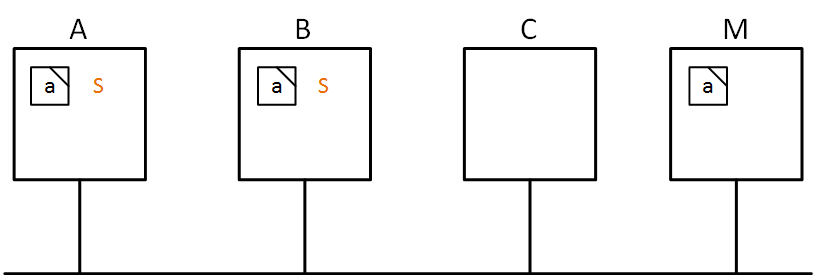
\includegraphics[width=.5\textwidth]{res/mesi_04}
		\caption{A liest von Adresse a, das führt zu Anfrage an alle, B sendet Daten.}
		\label{pic:mesi04}
	\end{center}
\end{figure} 

\begin{description}
	\item[False Sharing] gemeinsame Speicherzelle, obwohl sich die Daten darin nicht überlappen
\end{description}

Im ZSP von B:
\begin{figure}[H]
	\begin{center}
		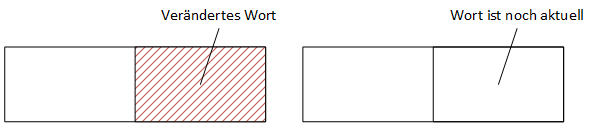
\includegraphics[width=.5\textwidth]{res/false_sharing_01}
		\caption{Speicherzeile für Adresse a.}
		\label{pic:falsesharing}
	\end{center}
\end{figure} 
False Sharing führt unnötig häufig zu Modus I.\\
\\
Daten, die nebeneinander verwendet werden, sollten in verschiedenen Speicherzeilen liegen.\\
\\
Verhalten mit getAndSet:\\
getAndSet(c, b, true)\\
Dabei ausgeführte Aktionen:
\begin{enumerate}
	\item c lesen
	\item b schreiben
	\item c schreiben
\end{enumerate}
\begin{figure}[H]
	\begin{center}
		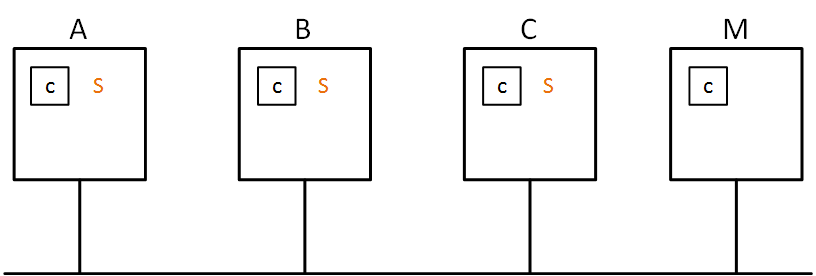
\includegraphics[width=.5\textwidth]{res/mesi_05}
		\caption{Zustand vorher.}
		\label{pic:mesi05}
	\end{center}
\end{figure} 
\begin{figure}[H]
	\begin{center}
		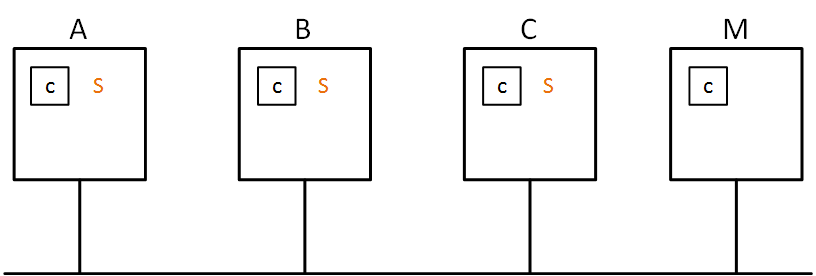
\includegraphics[width=.5\textwidth]{res/mesi_06}
		\caption{A führt (1) aus, Wert von c in ZSP von A ist bereits aktuell, keine Änderung.}
		\label{pic:mesi06}
	\end{center}
\end{figure} 
\begin{figure}[H]
	\begin{center}
		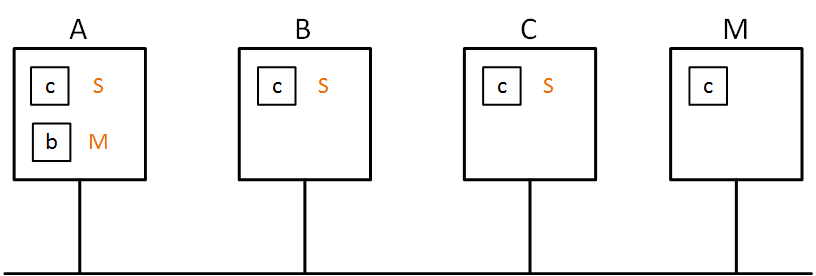
\includegraphics[width=.5\textwidth]{res/mesi_07}
		\caption{A führt (2) aus.}
		\label{pic:mesi07}
	\end{center}
\end{figure} 
\begin{figure}[H]
	\begin{center}
		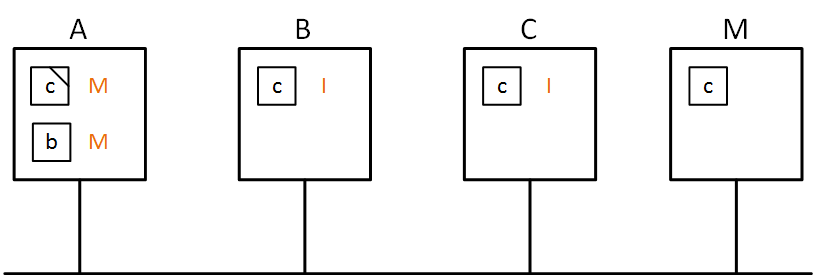
\includegraphics[width=.5\textwidth]{res/mesi_08}
		\caption{A führt (3) aus.}
		\label{pic:mesi08}
	\end{center}
\end{figure} 
\begin{figure}[H]
	\begin{center}
		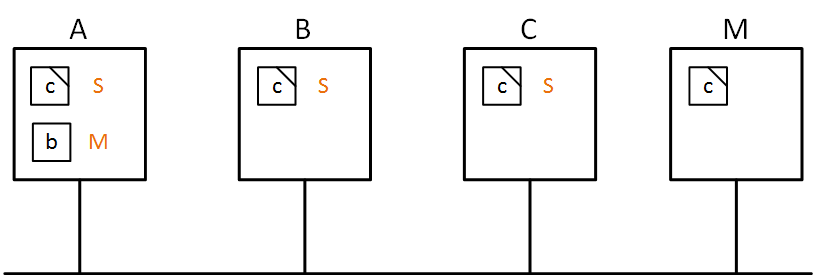
\includegraphics[width=.5\textwidth]{res/mesi_09}
		\caption{B führt (1) aus.}
		\label{pic:mesi09}
	\end{center}
\end{figure} 
\begin{figure}[H]
	\begin{center}
		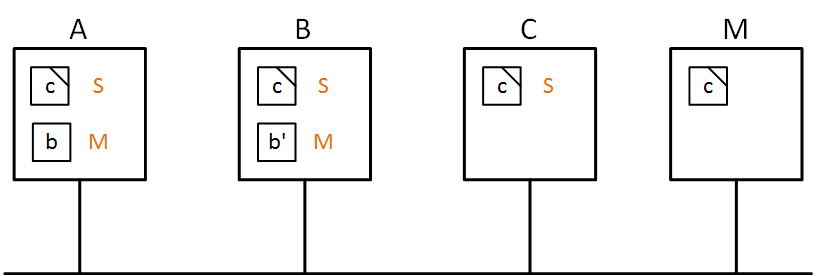
\includegraphics[width=.5\textwidth]{res/mesi_10}
		\caption{B führt (2) aus.}
		\label{pic:mesi10}
	\end{center}
\end{figure} 
\begin{figure}[H]
	\begin{center}
		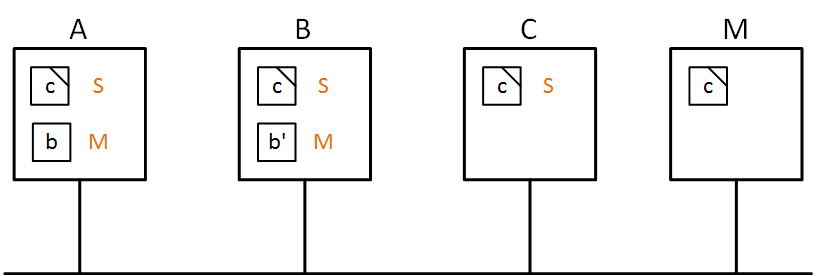
\includegraphics[width=.5\textwidth]{res/mesi_11}
		\caption{B führt (3) aus, keine Änderung, denn der Wert in c verändert sich nicht dabei.}
		\label{pic:mesi11}
	\end{center}
\end{figure} 

Alle getAndSet-Aufrufe der Warteschleife können ohne BUS-Zugriff abgearbeitet werden.

\section{Bäckerei-Algorithmus}
\begin{description}
	\item[Bäckerei-Algorithmus (engl bakery algorithm)] von Leslie Lamport 1974 publiziert; Implementierung von Sperren mit atomaren Registern.
\end{description}

Analogie: Jeder, der (in Amerika) eine Bäckerei betritt, zieht zuerst eine laufende Nummer. Der Kunde mit der niedrigsten Nummer wird als nächste bedient.\\
\\
Pseudocode mit einer Sperre:\\
\begin{lstlisting}[escapeinside={(*}{*)}]
Typ Thread ID = {0, ..., n - 1}; // n Threads
volatile flag: boolean[ThreadID]; // initialisiert mit false
volatile label: long[ThreadID]; // initialisiert mit 0
Prozedur belegen():
    int i := Nummer des aufrufenden Threads;
    flag[i] := true;
    label[i] := max(label[0], ..., label[n - 1]) + 1;
    Warte solange (* $\exists k \neq i : \text{flag}[k] \land \left(\text{label}[k], k\right) <_\text{lex} \left(\text{label}[i], i\right)$ *)
Prozedur freigeben():
    flag[Nummer des aufrufenden Threads] := false;
\end{lstlisting}
\textbf{Behauptung:} Der Bäckerei-Algorithmus hat die Fortschritt-Eigenschaft.\\
\textbf{Beweis:} Der Thread i mit dem kleinsten Paar (label[i], i) wartet nicht. Es gibt so ein i, denn $<_\text{lex}$ ist eine Wohlordnung. Damit hat jede nicht-leere Menge ein kleinstes Element.\\
\\
\textbf{Behauptung:} Der Bäckerei-Algorithmus ist FCFS (First Come First Serve).\\
\textbf{Beweis:} Falls Thread i den Torweg verlässt, bevor Thread j ihn betritt, dann gilt:
\begin{align*}
	& w_i\left(label[i], v\right) \rightarrow\\
	& r_j\left(label[i], v\right) \rightarrow\\
	& w_j\left(label[j], v'\right) \text{ mit } v < v'\\
	& r_j\left(flag[i], true\right)
\end{align*}
Dabei bedeutet $w_i\left(label[i], v\right)$: Schreibzugriff von Thread $i$ auf die Variable $label[i]$; der geschriebene Wert ist v.\\
Es gilt $flag[i] \land \left(flat[i], i\right) <_\text{lex} \left(label[j], j\right)$.\\
Aus Fortschritt und FCFS folgt Fairness.\\
\\
\textbf{Behauptung:} Der Bäckerei-Algorithmus erfüllt gegenseitigen Ausschluss.\\
\textbf{Beweis:} Durch Widerspruch (grundsätzliche Methode: Man behauptet, zwei Threads seien simulatan im kritischen Bereich. Herbeiführung von Widerspruch). Angenommen Threads i und j sind nebeneinander im kritischen Bereich. O.B.d.A. gilt: $\left(label[i], i\right) <_\text{lex} \left(label[j], j\right)$. Sobald Thread j die Warteschleife verlassen hat, gilt:
\begin{equation*}
	flag[i] = false \text{ (1)}
\end{equation*}
oder
\begin{equation*}
	\left(label[j], j\right) <_\text{lex} \left(label[i], i\right) \text{ (2)}
\end{equation*}
Die Werte von i und j sind fest. Der Wert von label[j] ändert sich nicht mehr bis zum Betreten des kritischen Bereichs. Der Wert von label[i] kann höchstens größer werden.\\
Wenn also (2) beim Verlassen der Warteschleife gilt, dann auch im kritischen Bereich. Widerspruch!\\
Also gilt (1). Deswegen 
\begin{align*}
&	r_j\left(\text{label}[i], \_\right) \rightarrow \text{ (\_: gelesener Wert ist irrelevant)}\\
&	w_j\left(\text{label}[j], v\right) \rightarrow\\
&	r_j\left(\text{flag}[i], false\right) \rightarrow\\
&	w_i\left(\text{flag}[i], true\right) \rightarrow\\
&	r_i\left(\text{label}[j], v\right) \rightarrow\\
&	w_i\left(\text{label}[i], v'\right)
\end{align*}
mit $v < v'$, also $\text{label}[j] < \text{label}[i]$. Widerspruch!\\
\\
Nachteil: Falls nur atomare Lese- und Schreib-Operationen zur Verfügung stehen ("`atomare Register"'), sind für n Threads Lese- und Schreibzugriffe auf mindestens n Speicherzellen notwendig (Burns/Lynch 1993).\\
Grund: Jeder Thread benötigt eine Speicherzelle, auf die nur er schreibt. Sonst kann ein anderer Thread das überschreiben, was ein anderer geschrieben hat.\\
Es muss mindestens n + 1 unterscheidbare Zustände geben: 
\begin{enumerate}
	\item kein Thread befindet sich im kritischen Bereich
	\item Thread i befindet sich im kritischen Bereich
\end{enumerate}
\chapter{Transactional Memory}

\begin{thebibliography}{x}
\bibitem{HERLIHY}Maurice Herlihy, Nir-Shavit: "`The Art of Multiprocessor Programming"', Morgan Kaufmann, 2008.
\bibitem{LIN}Kalvin Lin, Larry Snyder: "`Principles of Parallel Programming"', Addison Wesley.
\bibitem{ANDREWS}Greg Andrews: "`Concurrent Programming"', Addison Wesley, 1991.
\bibitem{GOETZ}Brian Goetz, u.a.: "`Java Concurrency in Practice"', Addison Wesley.
\end{thebibliography}

\end{document}